\documentclass[12pt]{article}

\usepackage{amsmath,amsfonts,amsthm}
\usepackage{bm}
\usepackage{natbib}
\usepackage{fullpage}
\usepackage{graphicx}
\usepackage{float}

\newcommand{\yt}{y_T}
\newcommand{\yc}{y_C}
\newcommand{\yti}{y_{Ti}}
\newcommand{\yci}{y_{Ci}}
\newcommand{\nt}{n_T}
\newcommand{\nc}{n_C}
\newcommand{\tsd}{\hat{\tau}_{sd}}
\newcommand{\tbar}{\bar{\tau}}
\newcommand{\tht}{\hat{\tau}_{ht}}
\newcommand{\pred}{\hat{y}}
\newcommand{\resid}{R}
\newcommand{\vht}{\hat{V}_{ht}}
\newcommand{\thipwi}{\hat{\tau}_i^{ipw}}
\newcommand{\predc}{\hat{y}_C(\cdot)}
\newcommand{\predt}{\hat{y}_T(\cdot)}
\newcommand{\predcx}{\hat{y}_C(\bm{x}_i)}
\newcommand{\predtx}{\hat{y}_T(\bm{x}_i)}
\newcommand{\thipw}{\hat{\tau}^{IPW}}
\newcommand{\thim}{\hat{\tau}_i^m}
\newcommand{\thm}{\hat{\tau}^m}
\newcommand{\hmi}{\hat{m}_i}
\newcommand{\EE}{\mathbb{E}}
\newcommand{\predcr}[1]{\hat{y}_C^{rem}(#1)}
\newcommand{\predtr}{\hat{y}_T^{rem}(\cdot)}
\newcommand{\predcxr}{\tilde{x}_i}
\newcommand{\predtxr}{\hat{y}_T^{rem}(\bm{x}_i)}


\newcommand\independent{\protect\mathpalette{\protect\independenT}{\perp}}
\def\independenT#1#2{\mathrel{\rlap{$#1#2$}\mkern2mu{#1#2}}}

\DeclareMathOperator*{\argmin}{arg\,min}



\title{Rebar+LOOP=Awesome}


\begin{document}
\maketitle
\section{Introduction}
A/B tests etc


\section{Methodological Background}

\subsection{Causal Inference from Experiments}
Consider a randomized experiment to estimate the average
effect of a binary treatment $T$ on an outcome $Y$.
Following \citet{neyman:1923} and \citet{rubin1974estimating}, for subject $i=1,\dots,N$,
let potential outcomes $\yti$ and $\yci$ represent the outcome value
$Y_i$ that $i$ would have exhibited if he or she had (perhaps
counterfactually) been assigned to treatment, $T_i=1$ or control,
$T_i=0$.
Then define the treatment effect for $i$ as $\tau_i=\yti-\yci$; our goal will be
to estimate the average treatment effect (ATE), $\tbar\equiv\sum_i\tau_i/N$.

If both $\yci $ and $\yti $ were known for each subject $i$,
statistical modeling would be unnecessary---researchers could
calculate $\tbar $ exactly, without error, % as the
%difference between $\bar{\yt}=\sum_i\yti/N$ and
%$\bar{\yc}=\sum_i\yci/N$, or equivalently
by simply averaging observed $\tau$.
In practice, we never observe both $\yci$ and $\yti$.
Instead, we rely on the experimental setup to estimate and infer
causation.
Since the treatment group is a random sample of
the $N$ participants, survey sampling literature provides design-based
unbiased estimators of the mean of $\yt$ based on observed $Y$ in the treatment group
and the known distribution of $T$.
These estimators, and their associated inference, depend only on the
experimental design, and not on modeling assumptions.
Likewise, the survey sampling literature suggests analogous unbiased,
design-based estimators for the mean of $\yc$ based on observed $Y$ values in
the control group, which is itself a random sample.
The survey sample structure of randomized experiments allows us to
infer counterfactual potential outcomes (at least on average) and estimate $\tbar$ as if
$\tau_i$ were available for each $i$, albeit with sampling error.

We will use this framework to analyze the 22 TestBed experiments.
These are examples of ``Bernoulli experiments,'' in
which each $T_i$ is an
independent Bernoulli trial: $Pr(T_i=1)\equiv p_i$, with $0<p_i<1$, and
$T_i\independent T_j \text{ if } i\ne j$.
In the TestBed experiments,
$p_i=1/2$ for all $i$.
Observed outcomes are a function of treatment assignment and
potential outcomes:
\begin{equation*}
  Y_i=T_i\yti+(1-T_i)\yci=\yci+\tau_iT_i.
\end{equation*}
In this model, $Y_i$ is only random due to its dependence on $T_i$;
$Y_i$ has a discrete distribution, with $Pr(Y_i=\yci)=1-p_i$,
$Pr(Y_i=\yti)=p_i$, and $Pr(Y_i=y')=0$ for any
$y'\not\in\{\yci,\yti\}$.
Since either $\yti$ or $\yci$ is unobserved, $Y_i$'s distribution is never known.
Along the same lines, let $M_i=T_i\yci+(1-T_i)\yti$, $i$'s unobserved
counterfactual outcome---when $i$ is treated, $M_i=\yci$ and when $i$
is in the control condition $M_i=\yti$.
Then $i$'s treatment effect may be expressed as $\tau_i=Y_i-M_i$ if
$i$ is in the treatment group or $\tau_i=M_i-Y_i$ if $i$ is in the
control group.
Although $M_i$ is, by definition, unobserved, it plays a central role in
causal inference, as does its expectation,
\begin{equation*}
m_i\equiv p_i\yci+(1-p_i)\yti
\end{equation*}
which will play a prominent role in the method we are proposing.

Under this model, estimation and inference about $\bar{\tau}$ is based on
the observed values of $Y$ and $T$.
Let
\begin{equation*}
U_i=\begin{cases}
\frac{1}{p_i} & T_i=1\\
-\frac{1}{1-p_i} & T_i=0
\end{cases}
\end{equation*}
be subject $i$'s signed inverse probability weights.
Note that $\EE U_i=0$, and $\EE U_iY_i=\tau_i$.
(To see this, note that when $T=1$, with probability $p_i$,
$Y_i=\yti$ and $U_iY_i=\yti/p_i$; when $T=0$, with probability
$1-p_i$, $U_iY_i=-yci/(1-p_i)$).
Then $U_iY_i$ may be thought of as an unbiased estimate of $\tau_i$, and $\thipw=\sum_iU_iY_i/N$ is an unbiased estimate
of $\bar{\tau}$.
In fact, $\thipw$ is identical to the ``Horvitz-Thompson'' estimator
of, e.g., \citet{aronowMiddleton}
\begin{equation*}
\thipw=\frac{1}{N}\displaystyle\sum_{i\in\mathcal{T}}
\frac{Y_i}{p_i}-\frac{1}{N}\displaystyle\sum_{i\in\mathcal{C}}\frac{Y_i}{1-p_i}
\end{equation*}
where $\mathcal{C} = \{i | T_i = 0\}$ is the control group and
$\mathcal{T} = \{i | T_i = 1\}$ is the treatment group.
This, in turn, is the difference between the Horvitz-Thomson
estimates of $\bar{\yt}$ and $\bar{\yc}$ \citep{horvitzThompson}.

The sampling variance of $\thipw$ proceeds from the same principals:
the variance of $U_iY_i$ is
\begin{equation}\label{eq:varTauHat1}
V(U_iY_i)=\left(\yti\sqrt{\frac{1-p_i}{p_i}}+\yci\sqrt{\frac{p_i}{1-p_i}}\right)^2=\frac{m_i^2}{p_i(1-p_i)}
\end{equation}
and, since  subjects' treatment assignments are mutually independent,
$V(\thipw)=1/N^2\sum_im_i^2/\{p_i(1-p_i)\}$.
Since $\yti $ and $\yci $ are never simultaneously observed,
$V(\thipw)$ is not identified; however, it may be bounded in expectation,
as $\hat{V}(\thipw)=\sum_iU_i^2Y_i^2/N^2$:
$\EE\hat{V}(\thipw)\le V(\thipw)$.
(See \citealt{aronowMiddleton} for equivalent expressions for more
general experimental designs.)

Classical survey sampling theory implies that $\thipw$ is
asymptotically normal, with asymptotic variance of at most
$\hat{V}(\thipw)$, so Wald-type confidence intervals of the form
$\thipw\pm z_{\alpha/2}\hat{V}(\thipw)^{1/2}$ achieve at least nominal coverage
in large samples.
These guarantees hold regardless of the distribution of
$\{\yc,\yt\}$---they depend only on the experimental design.



\subsection{Design-Based Covariate Adjustment}

The reason for error in estimating $\hat{\tau}$, is our inability to observe counterfactual
potential outcomes $M$.
As we've seen, randomized trials, coupled with design-based estimators
like $\thipw$, use comparison groups and survey sampling theory to
fill in this missing information.
Baseline covariates---a vector $\bm{x}_i$ of data for subject $i$
gathered prior to treatment randomization---may provide an alternative
strategy.
To see how, say a researcher had constructed algorithms $\predcx$ and
$\predtx$ designed to predict $\yc$ and $\yt$, respectively, from
$\bm{x}$.
Then, if $\hat{M}_i$ is an estimate of $i$'s missing counterfactual,
either $\predcx$ or $\predtx$, then $Y_i-\hat{M}_i$ (if $T_i=1$) or $\hat{M}_i-Y_i$ (if $T_i=0$)
may be considered estimates for $\tau_i$.
In general, the bias of algorithms such as $\predc$ and
$\predt$, will be unknown, so these effect estimates may be inadvisable.
On the other hand, imperfect or potentially biased predictions of
potential outcomes can, \emph{when combined with randomization}, yield
substantial benefits.

The approach we will take to combining covariate adjustment with
randomization follows \citet{loop}, as will its presentation here.
It has antecedents in \citet{rosenbaum2002covariance},
\citet{aronowMiddleton}, \citet{wager2016high}, and \citet{tame}.
In a Bernoulli experiment, note that
\begin{align*}
U_i(Y_i-m_i)&\\
&=\begin{cases}
\frac{1}{p_i}(\yti-p_i\yci-(1-p_i)\yti)&T_i=1\\
-\frac{1}{1-p_i}(\yci-p_i\yci-(1-p_i)\yti)&T_i=0 \end{cases}\\
&=\begin{cases}
\frac{p_i(\yti-\yci)}{p_i}&T_i=1\\
\frac{(1-p_i)(\yti-\yci)}{1-p_i}&T_i=0
\end{cases}\\
&=\tau_i
\end{align*}.
This suggests using predictions $\predcx$ and $\predtx$, to estimate $m_i$ as
$\hmi$,
and estimating $\tau_i$ as
\begin{equation*}
\thim\equiv U_i(Y_i-\hmi)
\end{equation*}

It turns out that $\thim$ is unbiased if prediction algorithms $\predc$ and $\predt$
are constructed in such a way that
\begin{equation}\label{eq:indPred}
\{\predcx,\predtx\}\independent T_i.
\end{equation}
Since $\bm{x}_i\independent T_i$ by design, (\ref{eq:indPred}) is
tantamount to requiring that $T_i$, and variables such as $Y_i$ that
depend on it, play no role in constructing prediction algorithms $\predc$ and
$\predt$.
%This requirement will be the focus of this paper's contributions.

Under (\ref{eq:indPred}), $\thim$ is indeed unbiased:
\begin{equation}
\EE \thim=\EE U_iY_i+\EE U_i\hmi=\EE U_iY_i+\EE U_i\EE\hmi=\EE
U_iY_i=\tau_i
\end{equation}
where we use the facts that $\EE U_i=0$ and $\EE U_iY_i=\tau_i$.
Finally, define ATE estimate
\begin{equation} \label{eq:thm}
\thm=\frac{1}{N}\displaystyle\sum_{i=1}^N
\thim=\frac{1}{N}\displaystyle\sum_{i=1}^N
\frac{T_i(Y_i-\hmi)}{p_i}-\frac{(1-T_i)(Y_i-\hmi)}{1-p_i}
\end{equation}
The unbiasedness of $\thm$ for $\bar{\tau}$ follows from the
unbiasedness of each of its summands, $\thim$ for $\tau_i$.

Crucially, this unbiasedness holds even if predictions $\predcx$ and $\predtx$ are biased; prediction algorithms $\predc$ and $\predt$ need not be unbiased, consistent, or correct in any sense.
As long as $\predcx$ and $\predtx$ are constructed to be independent
of $T_i$, $\thim$ will be unbiased.
The same cannot be said for regression-based covariance
adjustment, the common technique of regressing $Y$ on $T$ and $\bm{x}$
\citep{freedman2008regression}.

The goal of the covariate adjustment in $\thim$ is to estimate average
effects with greater precision;
its success in this regard depends on the predictive accuracy of $\predcx$ and $\predtx$.
\citet{loop} show that
\begin{equation}
V(\thim|\hmi)=\frac{(\hmi-m_i)^2}{p_i(1-p_i)}
\end{equation}
Accurate predictions of $\yci$ and $\yti$, and hence of $\hmi$, yield precise estimation of $\tau_i$.
On the other hand, inaccurate predictions (such that
$(\hmi-m_i)^2>m_i^2$) will decrease precision---though, again, without
causing bias.
%Note, however, that predictive accuracy of $\predc$ or $\predt$ does not impact bias.
The sampling variance of $\thm$ depends on the dependence structure of
$\hat{m}$, and will be discussed in the following two sections.

Under this framework, successful covariate adjustment
requires predictions $\predcx $ and $\predtx $ that are accurate and
independent of $T$.
To satisfy the independence condition, $i$'s outcome $Y_i$, which is a
function of $T$, cannot play a role in the construction of the algorithms $\predc$ and
$\predt$; they must be fit using other data.
Recent literature proposes two solutions to this problem.
 One approach \citep{rebarEDM} suggests
estimating prediction algorithm $\predc $ for all participants in the
experiment using an entirely separate dataset: covariate and outcome data from subjects
that were not part of the randomized experiment.
A second approach \citep{loop} fits a separate algorithm for each
experimental participant $i$, using data from experimental units other
than $i$.
The following two subsections will review these two approaches in some
depth.
The remainder of the paper will discuss their combination.

\subsection{Auxiliary Data: the Remnant from an Experiment}\label{sec:intro.remant}

Modern field trials are often conducted within a very data-rich
context, in which high-dimensional and rich covariate data is
automatically, or already, collected for all experiment participants.
For instance, in the TestBed experiments, system administrators have
access to log data for every problem and skill builder each
participating student worked before the onset of the experiment.
In other contexts, such as healthcare or education, rich
administrative data is available.
In fact, these covariates are available for a much wider population
than just the experimental participants---in the TestBed case, there
is log data for all ASSISTments users.
In healthcare or education examples, administrative data is available
for every student or patient in the system, not just for those who
were randomized to a treatment or control condition.
Often, as in the TestBed case, the outcome variable $Y$ is also drawn from administrative or
log data.
We refer to subjects within the same data system in which the
experiment took place---i.e. for whom covariate and outcome data are
available---but who were not part of the experiment, as the ``remnant'' from the experiment.
The remnant from a TestBed experiment consists of all ASSISTments
users for whom log data is available but who did not participate in
the experiment.

Clearly, pooling data from the remnant with data from the experiment
undermines the benefits and justification for randomization.
On the other hand, \citet{rebarEDM} argues that data from the remnant
can play a role in covariate adjustment.
Specifically, analysts may fit models $\predcr$ and $\predtr$ to data
from the remnant, and use those models, in conjunction with
experimental participants' own covariates $\bm{x}$, to predict their
experimental outcomes as $\predcxr$ and $\predtxr$.%and use those
% predictions to estimate $\hmi $.\footnote{\citet{rebarEDM} used a
%   slightly different causal formalism, but its central ideas transfer
%   immediately to our case.}
When the experiment in question is testing a novel intervention, every
member of the remnant essentially experienced the control
condition---in that case, data are only available to predict $\yc$,
and not $\yt$.

Since the models $\predcr $ and $\predtr $ are fit using data from a
separate sample from the experiment, and $\bm{x}\independent T$ by
design, predictions $\predcxr $ and $\predtxr $ satisfy the
independence criterion (\ref{eq:indPred}).
Furthermore, they may be fit and assessed in any way, as
long as only remnant data is used.
This process can be iterative, so that an analyst may fit a candidate
model, assess its performance (perhaps with $k-$fold
cross-validation), modify the model, and repeat until suitable
performance is achieved.
This follows from the fact that inference proceeds from the
randomization of $T$, and models fit in the remnant are invariant to
$T$.
Any realization of the assignment vector $\bm{T}$ would have given
rise to precisely the same predictions $\predcxr $ and $\predtxr $.
The frequent problem of post-selection inference, which is exacerbated
when the dimension of $\bm{x}$ is large, does not apply here.

In principal, a researcher may plug $\predcxr$ and $\predtxr$ into formula
(\ref{eq:hatm}) for $\hmi$ to estimate $\thim$ and, hence, $\thm$.
Indeed, \citet{rebarEDM} used an analogous strategy to some success.
On the other hand, doing so incurs risk---when $\hmi$ is a poor
prediction of $m_i$, so that $(m_i-\hmi)^2>m_i^2$, covariance
adjustment using $\predcx$ and $\predtx$ increases sampling variance.
This will be the case if predictive models fit in the remnant
extrapolate poorly to the experimental sample---for instance, if the
distribution of $\bm{x}$, or the distribution of $\yc$ or $\yt$
conditional on $\bm{x}$, differ subsantially between the two samples.
To make matters worse, the performance of $\predcr$ and $\predtr$ in the
experimental sample---where it counts---may not be checked directly.
Once a researcher uses observed experimental outcomes $Y$ to select
$\predcr$ or $\predtr$, the resulting predictions $\predcx$ and
$\predtx$ may no longer be independent of $T$, violating
(\ref{eq:indPred}).

Another potential problem occurs when only the control condition
occurs in the remnant, so only $\predcr$ may be fit.
In those cases, we let $\hmi=\predtxr=\predcxr$ for all subjects.
Doing so may further increase squared prediction error $(m_i-\hmi)^2$.
Of course, a preliminary estimate of $\bar{\tau}$ is available from
the experimental data, but as before, incorporating experimental
outcomes into $\hat{m}$ induces a dependence between $\hat{m}$ and
$T$.

The remnant from an experiment is often much larger than the
experimental sample, and may provide fertile ground for predicting
potential outcomes, especially in the presence of rich
high-dimensional covariates.
However, absent methods to use experimental data to assess predictive
accuracy and account for possible treatment effects, covariance
adjustment using the remnant is risky.

\subsection{LOOP}

An additional risk of covariate adjustment, even when data from the remnant is not used, is the possibility of overfitting.  This is particularly a concern when there is a large number of covariates with little predictive power.  Overfitting may result in adjustments that harm rather than improve precision \citep{freedman2008regression, miratrix}.  This is a concern of \cite{loop}, and their LOOP estimator allows for automatic variable selection to avoid overfitting.  Importantly, \cite{loop} argue that LOOP will typically not harm precision and perform no worse than the simple difference estimator.

The LOOP estimator is a leave-one-out method that proceeds as follows.  For each $i$, we first drop observation $i$, and then use the remaining $N-1$ observations to construct prediction models for the control and treatment potential outcomes, denoted $\hat{y}^{(-i)}_C(\mathbf{x})$ and $\hat{y}^{(-i)}_T(\mathbf{x})$, respectively.  These models may be fit by any method, for example linear regression or random forests.  In particular, methods that allow for automatic variable selection, or other forms of dimensionality reduction or regularization to prevent overfitting may be used.

Next, following equation (\ref{eq:hatm}), we set
\begin{equation}
\hat{m}_i = p\hat{y}^{(-i)}_{C}(\mathbf{x}_i) + (1-p)\hat{y}^{(-i)}_{T}(\mathbf{x}_i)
\end{equation}
and the LOOP estimator is then given by $\hat{\tau}^m$ in (\ref{eq:thm}).  Note that here $\hat{m}_i \independent T_i$ due to the fact that $\hat{m}_i$ is computed without observation $i$.  It follows that $\hat{\tau}^m$ is unbiased.

\cite{loop} provide an estimate for the variance of the LOOP estimator.  Let
\begin{align}
\hat{E}_C = & \frac{1}{n_C}\sum_{i \in \mathcal{C}}(\hat{y}_{Ci} - y_{Ci})^2 \label{Echat}
\end{align}
and define $\hat{E}_T$ similarly.  Note $\hat{E}_C$ and $\hat{E}_T$ are leave-one-out cross validation mean squared errors.  The estimated variance is then given by
\begin{align}
\widehat{\mathrm{Var}}(\hat{\tau}) =  \frac{1}{N}\left[\frac{p}{1-p}\hat{E}_C + \frac{1-p}{p}\hat{E}_T + 2\sqrt{\hat{E}_C\hat{E}_T}\right]. \label{loopvarhat}
\end{align}
\cite{loop} note that (\ref{loopvarhat}) will typically be somewhat conservative.  This is due to the fact that $\mathrm{Var}(\hat{\tau})$ is unidentifiable, which itself derives from the fact that we only ever observe one potential outcome for each unit, and thus the correlation of the potential outcomes cannot be estimated.  Instead, a bound must be used.  This difficulty is not unique to the LOOP estimator; similar comments apply to the simple difference estimator \citep{aronow2014}.  Note also that
\begin{align}
\frac{1}{N}\left[\frac{p}{1-p}\hat{E}_C + \frac{1-p}{p}\hat{E}_T + 2\sqrt{\hat{E}_C\hat{E}_T}\right]
&\le
\frac{\hat{E}_C}{N(1-p)} + \frac{\hat{E}_T}{Np} \\
&\approx
\frac{\hat{E}_C}{n_C} + \frac{\hat{E}_T}{n_T} \label{t-test-like-variance}
\end{align}
which is similar in form to the variance estimate typically used in a two-sample $t$-test, namely $\frac{s^2_C}{n_C} + \frac{s^2_T}{n_T}$, where $s^2_C$ and $s^2_T$ denote the control group and treatment group sample variances.  In (\ref{t-test-like-variance}), $s^2_C$ and $s^2_T$ are replaced by $\hat{E}_C$ and $\hat{E}_T$.  In other words, the variances are replaced by the estimated mean squared errors of the imputations.

A special case of the LOOP estimator occurs when the potential outcomes are imputed by simply taking the mean of the observed  outcomes (after dropping observation $i$).  That is, we set
\begin{equation}
\hat{y}^{(-i)}_C(\mathbf{x}) = \bar{y}^{(-i)}_{Ci}\equiv \frac{1}{|{\mathcal{C}\setminus i}|}\sum_{j \in \mathcal{C} \setminus i} y_{Cj}
\end{equation}
and similarly for $\hat{y}^{(-i)}_T(\mathbf{x})$.  Note that in this case the covariates are ignored.  It can be shown that when the potential outcomes are mean-imputed in this manner the LOOP estimator $\hat{\tau}^{m}$ is exactly equal to the simple difference estimator
\begin{equation}
\hat{\tau}^{SD} = \frac{1}{n_T}\sum_{i \in \mathcal{T}}Y_i - \frac{1}{n_C}\sum_{i \in \mathcal{C}}Y_i
\end{equation}
\citep{loop}.  Moreover, $\hat{E}_C = \frac{n_C}{n_C-1}s^2_C$ and $\hat{E}_T = \frac{n_T}{n_T-1}s^2_C$ and thus the variance estimate given by (\ref{t-test-like-variance}) is nearly identical to the ordinary $t$-test variance estimate.

In short, when using mean imputation for the potential outcomes, LOOP essentially simplifies to an ordinary $t$-test.  The effect estimate is identical, and the variance estimate is nearly identical.  This is highly reassuring.  Any imputation strategy that improves upon mean-imputation in terms of mean squared error will reduce the variance of the LOOP estimator relative to the simple difference estimator.  Most modern machine learning methods employ some form of regularization to guard against overfitting, and thus typically perform no worse, or at least not substantially worse, than mean-imputation.  Thus in practice there is relatively little risk that LOOP will hurt precision.









\section{Method}
Our goal is to construct a method that, like rebar, is able to exploit data in the remnant but, like LOOP, poses little risk of harming precision.

% Let $\hat{y}_C^{rem}(\mathbf{x})$ denote a model for the control potential outcomes fitted from data in the remnant, as described in Section \ref{sec:intro.remant}.  Now define
% \begin{equation}
% \tilde{x}_{i} \equiv \hat{y}_C^{rem}(\mathbf{x}_i)
% \end{equation}
% for each $i$ in the experiment.  The
Recall that
$\tilde{x}_{i}$ are the imputed control potential outcomes for the
participants in the experiment, using a predictive model
$\predcr{\cdot}$ fit in the remnant, and that
  %However, as the notation suggests,
$\tilde{x}_{i}$ may also be thought of simply as an additional
covariate, along with those in $\mathbf{x}_i$.
%Indeed, $\tilde{x}_i$ is simply a function of the other covariates.
we may therefore include $\tilde{x}_{i}$ as a covariate in LOOP.  We now discuss
three options for doing so.


% Importantly, because $\hat{y}_C^{rem}(\mathbf{x})$ is fitted using only data from the remnant, this function may be regarded as fixed when analyzing the experimental data.  We therefore emphasize again that $\tilde{x}_{i}$ may be treated formally just like any other covariate.  In particular,


\paragraph{Strategy 1:}
%We therefore additionally define
Define
\begin{equation}
\tilde{\mathbf{x}}_i \equiv (\tilde{x}_{i}, x_{i1}, x_{i2}, ..., x_{ip})
\end{equation}
or in other words, $\tilde{\mathbf{x}}_i$ is $\mathbf{x}_i$ augmented with $\tilde{x}_i$.

The most straight-forward option would be to run LOOP on the experimental data, but using the augmented set of covariates $\tilde{\mathbf{x}}$ instead of $\mathbf{x}$.  The hope is that by including $\tilde{x}_{i}$ we can implicitly exploit information in the remnant in much the same way that rebar does.  Moreover, by using LOOP, we also reduce the risk of accidentally hurting precision.

A few comments:
(1) For this option we would use random forests as the imputation strategy within LOOP, as suggested by \cite{loop}.  We refer to LOOP with random forests as LOOP-RF.
(2) $\tilde{x}_{i}$ is a function of the other covariates and thus, in at least some sense, does not contain any additional information.  However, the function $\hat{y}_C^{rem}(\mathbf{x})$  is fitted on the remnant, which may be much larger than the experimental sample, and thus $\hat{y}_C^{rem}(\mathbf{x})$ may be a more accurate imputation function than what we would be able to obtain using the experimental data alone.  In this sense, $\tilde{x}_{i}$ does contain additional information, which LOOP-RF can exploit by heavily weighting $\tilde{x}_{i}$ over the other covariates.
(3) If the imputations $\tilde{x}_{i}$ are poor, then LOOP-RF may simply downweight or effectively ignore them.  In particular, poor imputations from the remnant should not harm precision.
(4) Biased imputations can still be helpful.  Importantly, because the $\tilde{x}_{i}$ are used as a covariate within LOOP-RF, they do not necessarily need to accurately impute the potential outcomes in the experimental sample; rather, it suffices that they are merely predictive of the potential outcomes.  If the experimental sample is systematically different from the remnant,  e.g., the potential outcomes in the experimental sample are on average higher than those in the remnant, the $\tilde{x}_{i}$ will still be useful as long as they are correlated with the experimental potential outcomes.
(5) We have implicitly assumed here that all units in the remnant are untreated, and the $\tilde{x}_{i}$ are imputed control potential outcomes.  In light of the previous comment (4), the $\tilde{x}_{i}$ may still be used as a covariate within LOOP-RF for predicting treatment potential outcomes, even if the $y_T$ differ from the $y_C$ due to a treatment effect, as long as $\tilde{x}$ is predictive of $y_T$.
(6) If the $\tilde{x}_{i}$ are highly accurate, using them as a covariate within a nonparametric method like a random forest may be statistically inefficient.  The random forest may effectively just add noise or bias.  It is this concern that motivates the next strategy.

\paragraph{Strategy 2:}
A second option would be to run LOOP on the experimental data, but using only $\tilde{x}_{i}$ as a predictor, and using linear regression instead of a random forest.  That is, for each $i$
\begin{equation}
\hat{y}_{Ci} = \hat{\beta}_{0C}^{(-i)} + \hat{\beta}_{1C}^{(-i)}\tilde{x}_{i}
\end{equation}
where  $\hat{\beta}_{0C}^{(-i)}$ and $\hat{\beta}_{1C}^{(-i)}$ are the coefficients from a regression of the observed $y_C$ on $\tilde{x}$, omitting observation $i$.  The expression for $\hat{y}_{Ti}$ would be analogous.

Strategy 2 may be preferable to strategy 1 when the $\tilde{x}_{i}$ are highly accurate imputations of $y_C$.  In that case, $\hat{\beta}_{1C}^{(-i)} \approx 1$
%and $\hat{\beta}_{0C}^{(-i)} \approx 0$
and $\hat{y}_{Ci} \approx \tilde{x}_{i}$.  In other words, the imputations from the remnant ``pass through'' the LOOP procedure largely unmodified, resulting in a rebar-like adjustment.  However, in contrast to rebar, poor imputations $\tilde{x}$ will not necessarily harm precision.  Consider the extreme case in which $\tilde{x}$ is pure noise.  We would then expect $\hat{\beta}_{1C}^{(-i)} \approx 0$ and $\hat{\beta}_{0C}^{(-i)} \approx \bar{y}^{(-i)}_{Ci}$ so that $\hat{y}_{Ci} \approx \bar{y}^{(-i)}_{Ci}$.  That is, we revert approximately to mean-imputation, and the final estimator is therefore approximately equal to the simple difference estimator.

\paragraph{Strategy 3:}

In practice it may not always be clear whether strategy 1 or 2 will perform better; it depends on the quality of the imputations $\tilde{x}$ as well as the predictive power of the covariates in the experimental sample.  Thus, a final option would be to combine strategies 1 and 2 by taking a weighted average.  Let $\hat{y}^{(-i, S1)}_{Ci}(\mathbf{\tilde{x}_i})$ and $\hat{y}^{(-i, S2)}_{Ci}(\tilde{x}_i)$ denote imputations from strategies 1 and 2, respectively.  We then let
\begin{equation}
\hat{y}^{(-i, S3)}_{Ci}(\mathbf{\tilde{x}_i}) = \alpha_i \hat{y}^{(-i, S1)}_{Ci}(\mathbf{\tilde{x}_i}) + (1-\alpha_i) \hat{y}^{(-i, S2)}_{Ci}(\tilde{x}_i)
\end{equation}
where $\alpha_i$ is given by
\begin{equation}
\alpha_i = \argmin_{\alpha \in [0,1]} \sum_{j \in \mathcal{C} \setminus i} \left[Y_j - \left(\alpha \hat{y}^{(-i, S1)}_{Cj}(\mathbf{\tilde{x}_j}) + (1-\alpha) \hat{y}^{(-i, S2)}_{Cj}(\tilde{x}_j) \right)\right]^2
\end{equation}









In this section, we examine the performance of ReLOOP using simulation. In particular, we consider how ReLOOP performs when varying sample size, the predictive power of the covariates, and the predictive power of the external predictions. Consider a randomized experiment in which there are $N$ subjects. The potential outcomes and covariates are generated from the following linear model:
\begin{align*}
a_i &= 2Z_{1,i} + Z_{2,i} + \delta_i \\
c_i &= \frac{ a_i }{ \sigma_{a} } \\
t_i &= c_i + 3
\end{align*}
where $\delta_i \sim \text{N}(0,\sigma_{gen}^2)$, $Z_{ij} \sim \text{Unif}(0,10)$, and $\sigma^2_{a} = \text{Var}(a_i) = \frac{500}{12} + \sigma_{gen}^2$. By generating our potential outcomes as above, we have defined our generative model such that the control potential outcomes have unit variance. We can alternatively write the observed outcome as:
\begin{align*}
Y_i &= 3 T_i + \frac{2}{\sigma_{a}}Z_{1,i} + \frac{1}{\sigma_{a}} Z_{2,i} + \epsilon_i
\end{align*}
where $\epsilon_i \sim \text{N}(0,\sigma_{gen}^2/\sigma^2_{a})$.
\\\\
For each observation, we also simulate external predictions $\tilde{t}_i$ and $\tilde{c}_i$ for $t_i$ and $c_i$ by taking the true $t_i$ or $c_i$ and adding a normally distributed noise term with mean 0 and standard deviation $\sigma_{ext}$.
\\\\
To reiterate, we wish to consider variations in sample size, the predictive power of the covariates, and the predictive power of the external predictions. Sample size is directly indexed with $N$. We can index the predictive power of the covariates using the control-side $R^2$:
\[ R_c^2 = 1 - \frac{ \sigma^2_{gen} }{ \sigma^2_{a} }. \]
Similarly, the predictive power of our external prediction $\tilde{c}_i$ is
\[ R^2_{p} = 1 - \frac{\sigma_{ext}^2}{\text{Var}( \tilde{c}_i )} = 1 - \frac{\sigma^2_{ext}}{1+\sigma^2_{ext}}. \]
Given a desired $R_c^2$ and $R^2_{p}$, we can calculate the corresponding values of $\sigma^2_{gen}$ and $\sigma^2_{ext}$ (note that $\sigma_{ext}^2$ and $\sigma_{gen}^2$ characterize the distribution of the external predictions and potential outcomes for a given set of covariates):
\begin{align*}
\sigma^2_{gen} &= \frac{1-R_c^2}{R_c^2}\times\frac{500}{12} \\
\sigma^2_{ext} &= \frac{1 - R^2_{p}}{R_p^2} .
\end{align*}
We perform three sets of simulations, in which we hold two of $N$, $R_c^2$, and $R^2_{p}$ constant and vary the third.  For each set of simulations, we compare the following methods:
\begin{enumerate}
	\item LOOP: uses the LOOP estimator including only the covariates $Z_1$ and $Z_2$
	\item LOOP with External Predictions: uses the LOOP estimator with external predictions as a covariate (in addition to $Z_1$ and $Z_2$)
	\item ReLOOP*: uses the LOOP estimator, with OLS as the imputation method. Only includes the external predictions as a covariate
	\item ReLOOP: interpolates between the previous two methods
\end{enumerate}
\noindent
We use the following simulation procedure. For a given set of $N$, $R_c^2$, and $R^2_{p}$, we perform $k = 1000$ trials. For each trial, we generate a set of potential outcomes, a treatment assignment vector, and external predictions for $t_i$ and $c_i$. We then produce an estimate of the variance of each method for that treatment assignment vector. Next, we average the estimated variance across the $k$ trials. Finally, we plot the average nominal variance for each method relative to the variance of the simple difference estimator.

\subsection{Varying Sample Size}
For this simulation, we hold the predictive power of the covariates and external predictions constant and vary the sample size $N = 30, 40, 50, 75, 100, 150, 200$. We consider four scenarios: (1) $R^2_p = 0.25, R^2_c = 0.25$; (2) $R^2_p = 0.75, R^2_c = 0.25$; (3) $R^2_p = 0.25, R^2_c = 0.75$; and (4) $R^2_p = 0.75, R^2_c = 0.75$:
\begin{figure}[H]
	\centering
	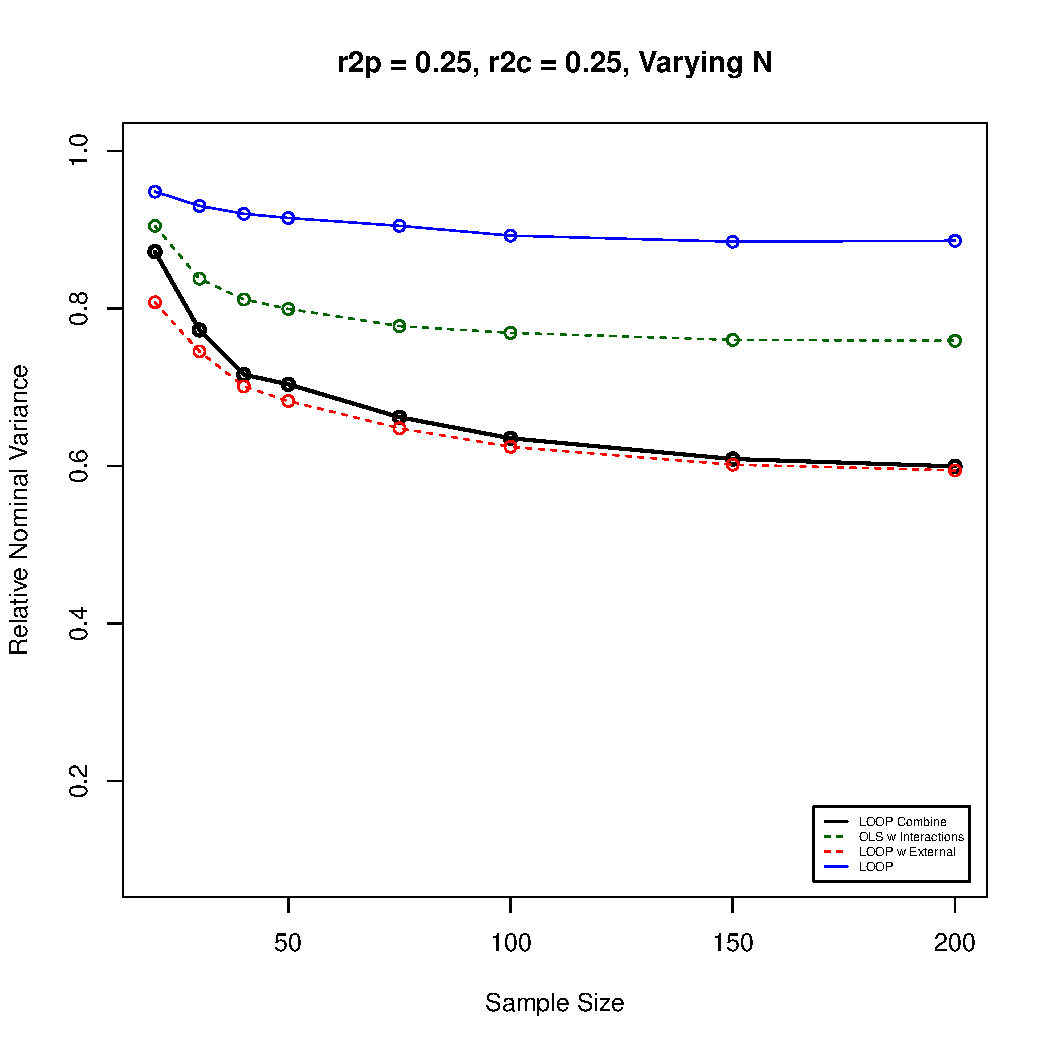
\includegraphics[width=.49\linewidth]{images/sampsize.pdf}
	\includegraphics[width=.49\linewidth,page = 2]{images/sampsize.pdf} \quad
	\smallskip
	\includegraphics[width=.49\linewidth,page = 3]{images/sampsize.pdf}
	\includegraphics[width=.49\linewidth,page = 4]{images/sampsize.pdf} \quad
	\caption{Top Left: $R^2_p = 0.25, R^2_c = 0.25$; Top Right: $R^2_p = 0.75, R^2_c = 0.25$; Bottom Left: $R^2_p = 0.25, R^2_c = 0.75$; Bottom Right: $R^2_p = 0.75, R^2_c = 0.75$}
\end{figure}
As we can see, when the predictive power is low for both the covariates and the external predictions ($R^2_p = 0.25, R^2_c = 0.25$), LOOP is outperformed by ReLOOP. Similarly, when the predictive power is high for both, ReLOOP outperforms LOOP. Even when $R^2_p$ is low and $R^2_c$ is high, the performance of ReLOOP quickly converges to the performance of LOOP. Finally we observe that ReLOOP does well at tracking the better performing component (and generally outperforms both components when the components perform similarly to each other).

\subsection{Varying Predictive Power of External Prediction}
For this simulation, we hold the predictive power of the covariates and sample size constant and vary $R^2_p = 0.05, 0.15, ..., 0.85, 0.95$. We consider four scenarios: (1) $N = 30, R^2_c = 0.25$; (2) $N = 30, R^2_c = 0.75$; (3) $N = 60, R^2_c = 0.25$; and (4) $N = 60, R^2_c = 0.75$:
\begin{figure}[H]
	\centering
	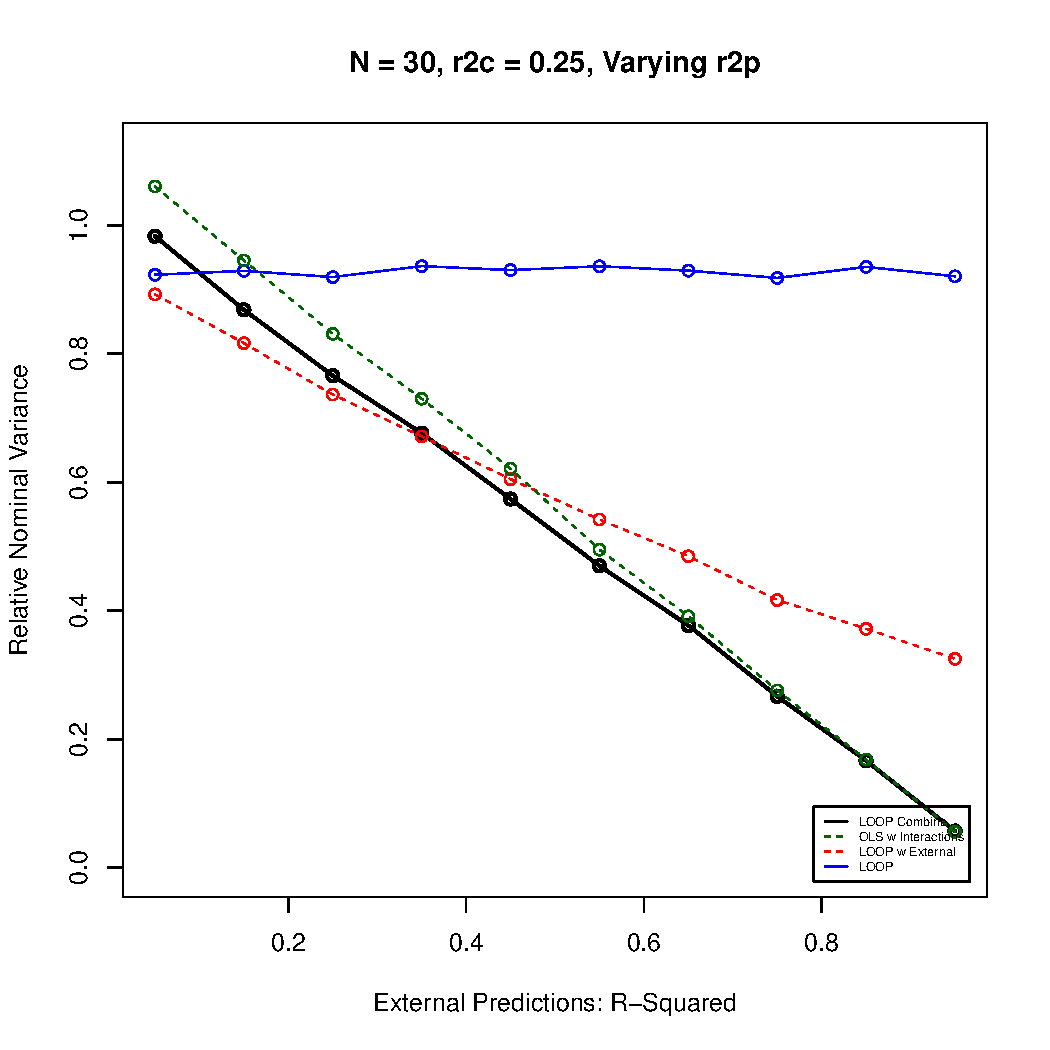
\includegraphics[width=.49\linewidth]{images/r2p.pdf}
	\includegraphics[width=.49\linewidth,page = 2]{images/r2p.pdf} \quad
	\smallskip
	\includegraphics[width=.49\linewidth,page = 3]{images/r2p.pdf}
	\includegraphics[width=.49\linewidth,page = 4]{images/r2p.pdf} \quad
	\caption{Top Left: $N = 30, R^2_c = 0.25$; Top Right: $N = 30, R^2_c = 0.75$; Bottom Left: $N = 60, R^2_c = 0.25$; Bottom Right: $N = 60, R^2_c = 0.75$}
\end{figure}
Once again, we observe that ReLOOP tends to perform at least as well as either component. This is particularly true for $N=60$, where ReLOOP closely follows (or drops below) the lower of the component lines. As expected, the three methods that incorporate the external predictions all improve as $R^2_p$ increases, while the performance of LOOP stays constant. We can see that ReLOOP is outperformed by LOOP when only when $R^2_p$ is much lower than $R^2_c$.

\subsection{Varying Predictive Power of Covariates}
For this simulation, we hold the predictive power of the external predictions and sample size constant and vary $R^2_c = 0.05, 0.15, ..., 0.85, 0.95$. We consider four scenarios: (1) $N = 30, R^2_p = 0.25$; (2) $N = 30, R^2_p = 0.75$; (3) $N = 60, R^2_p = 0.25$; and (4) $N = 60, R^2_p = 0.75$:
\begin{figure}[H]
	\centering
	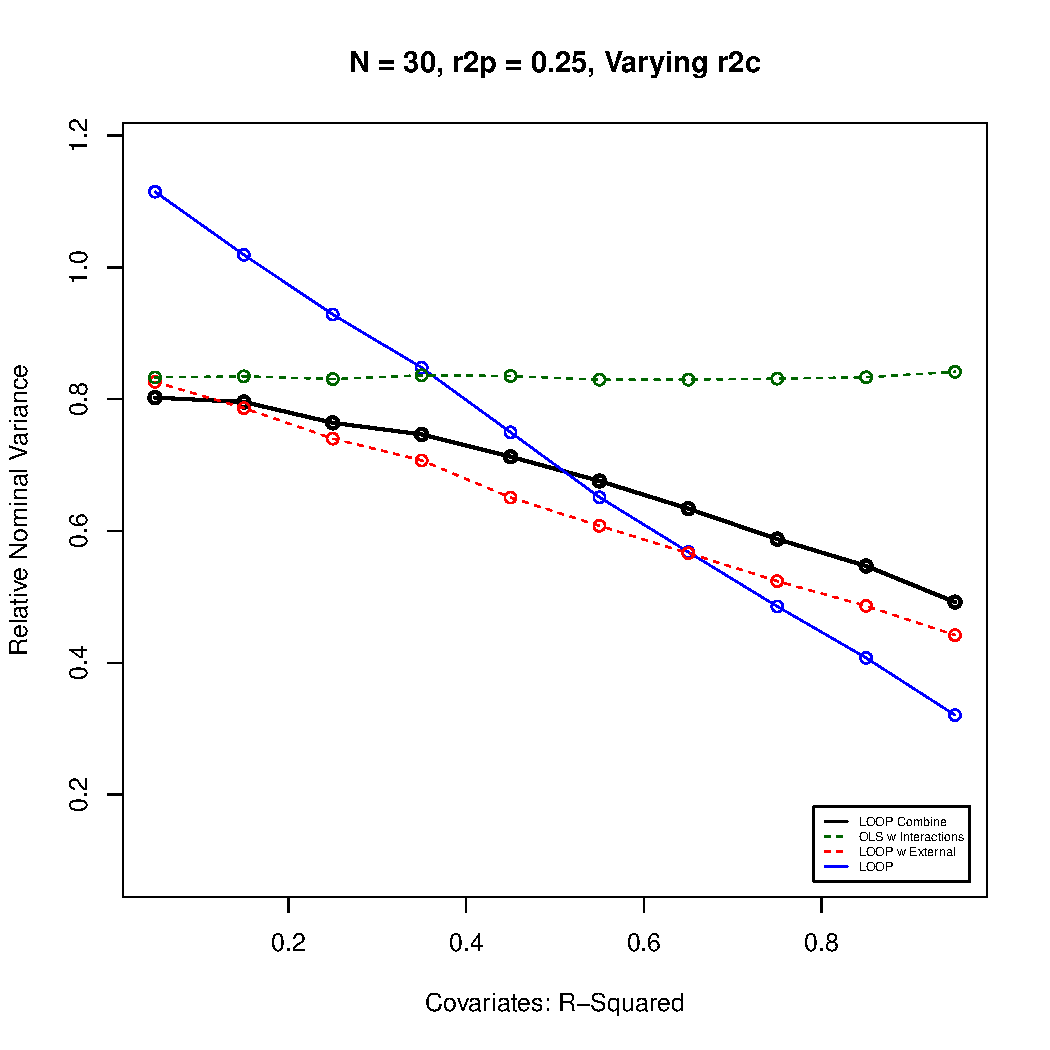
\includegraphics[width=.49\linewidth]{images/r2c.pdf}
	\includegraphics[width=.49\linewidth,page = 2]{images/r2c.pdf} \quad
	\smallskip
	\includegraphics[width=.49\linewidth,page = 3]{images/r2c.pdf}
	\includegraphics[width=.49\linewidth,page = 4]{images/r2c.pdf} \quad
	\caption{Top Left: $N = 30, R^2_p = 0.25$; Top Right $N = 30, R^2_p = 0.75$; Bottom Left $N = 60, R^2_p = 0.25$; Bottom Right: $N = 60, R^2_p = 0.75$}
\end{figure}
The performance of ReLOOP* stays constant, as the imputation method only incorporates the external predictions. The remaining methods all improve as $R^2_c$ increases. As before, we can see that ReLOOP tracks the better performing component well (especially when $N = 60$) and is only outperformed by LOOP when $R^2_c$ is much higher than $R^2_p$.






\bibliographystyle{plainnat}
\bibliography{rebarloop}

\end{document}
